%!TEX root = main.tex

\chapter{Theoretical background for lateral railway bridge dynamics}

This chapter contains theoretical basis of lateral railway bridge dynamics. The lateral dynamics of railway bridge is related to both structural dynamics and railway vehicle dynamics. This chapter aims to elaborate the basic concepts of both dynamics topics.

The railway vehicle dynamics part contains knowledge of \emph{Wheel-rail interface}, \emph{Lateral track irregularities} and \emph{Lateral movement of wheelsets}. The structural dynamics part will introduce knowledge about \emph{Bridge natural frequency}.

A brief introduction to the resonant interaction between bridge and vehicle is described in \emph{Lateral vehicle-bridge resonance}.

\section{Wheel-rail interface} 

\paragraph{Wheelset and track dimensions}

\begin{figure}[h!]
\centering
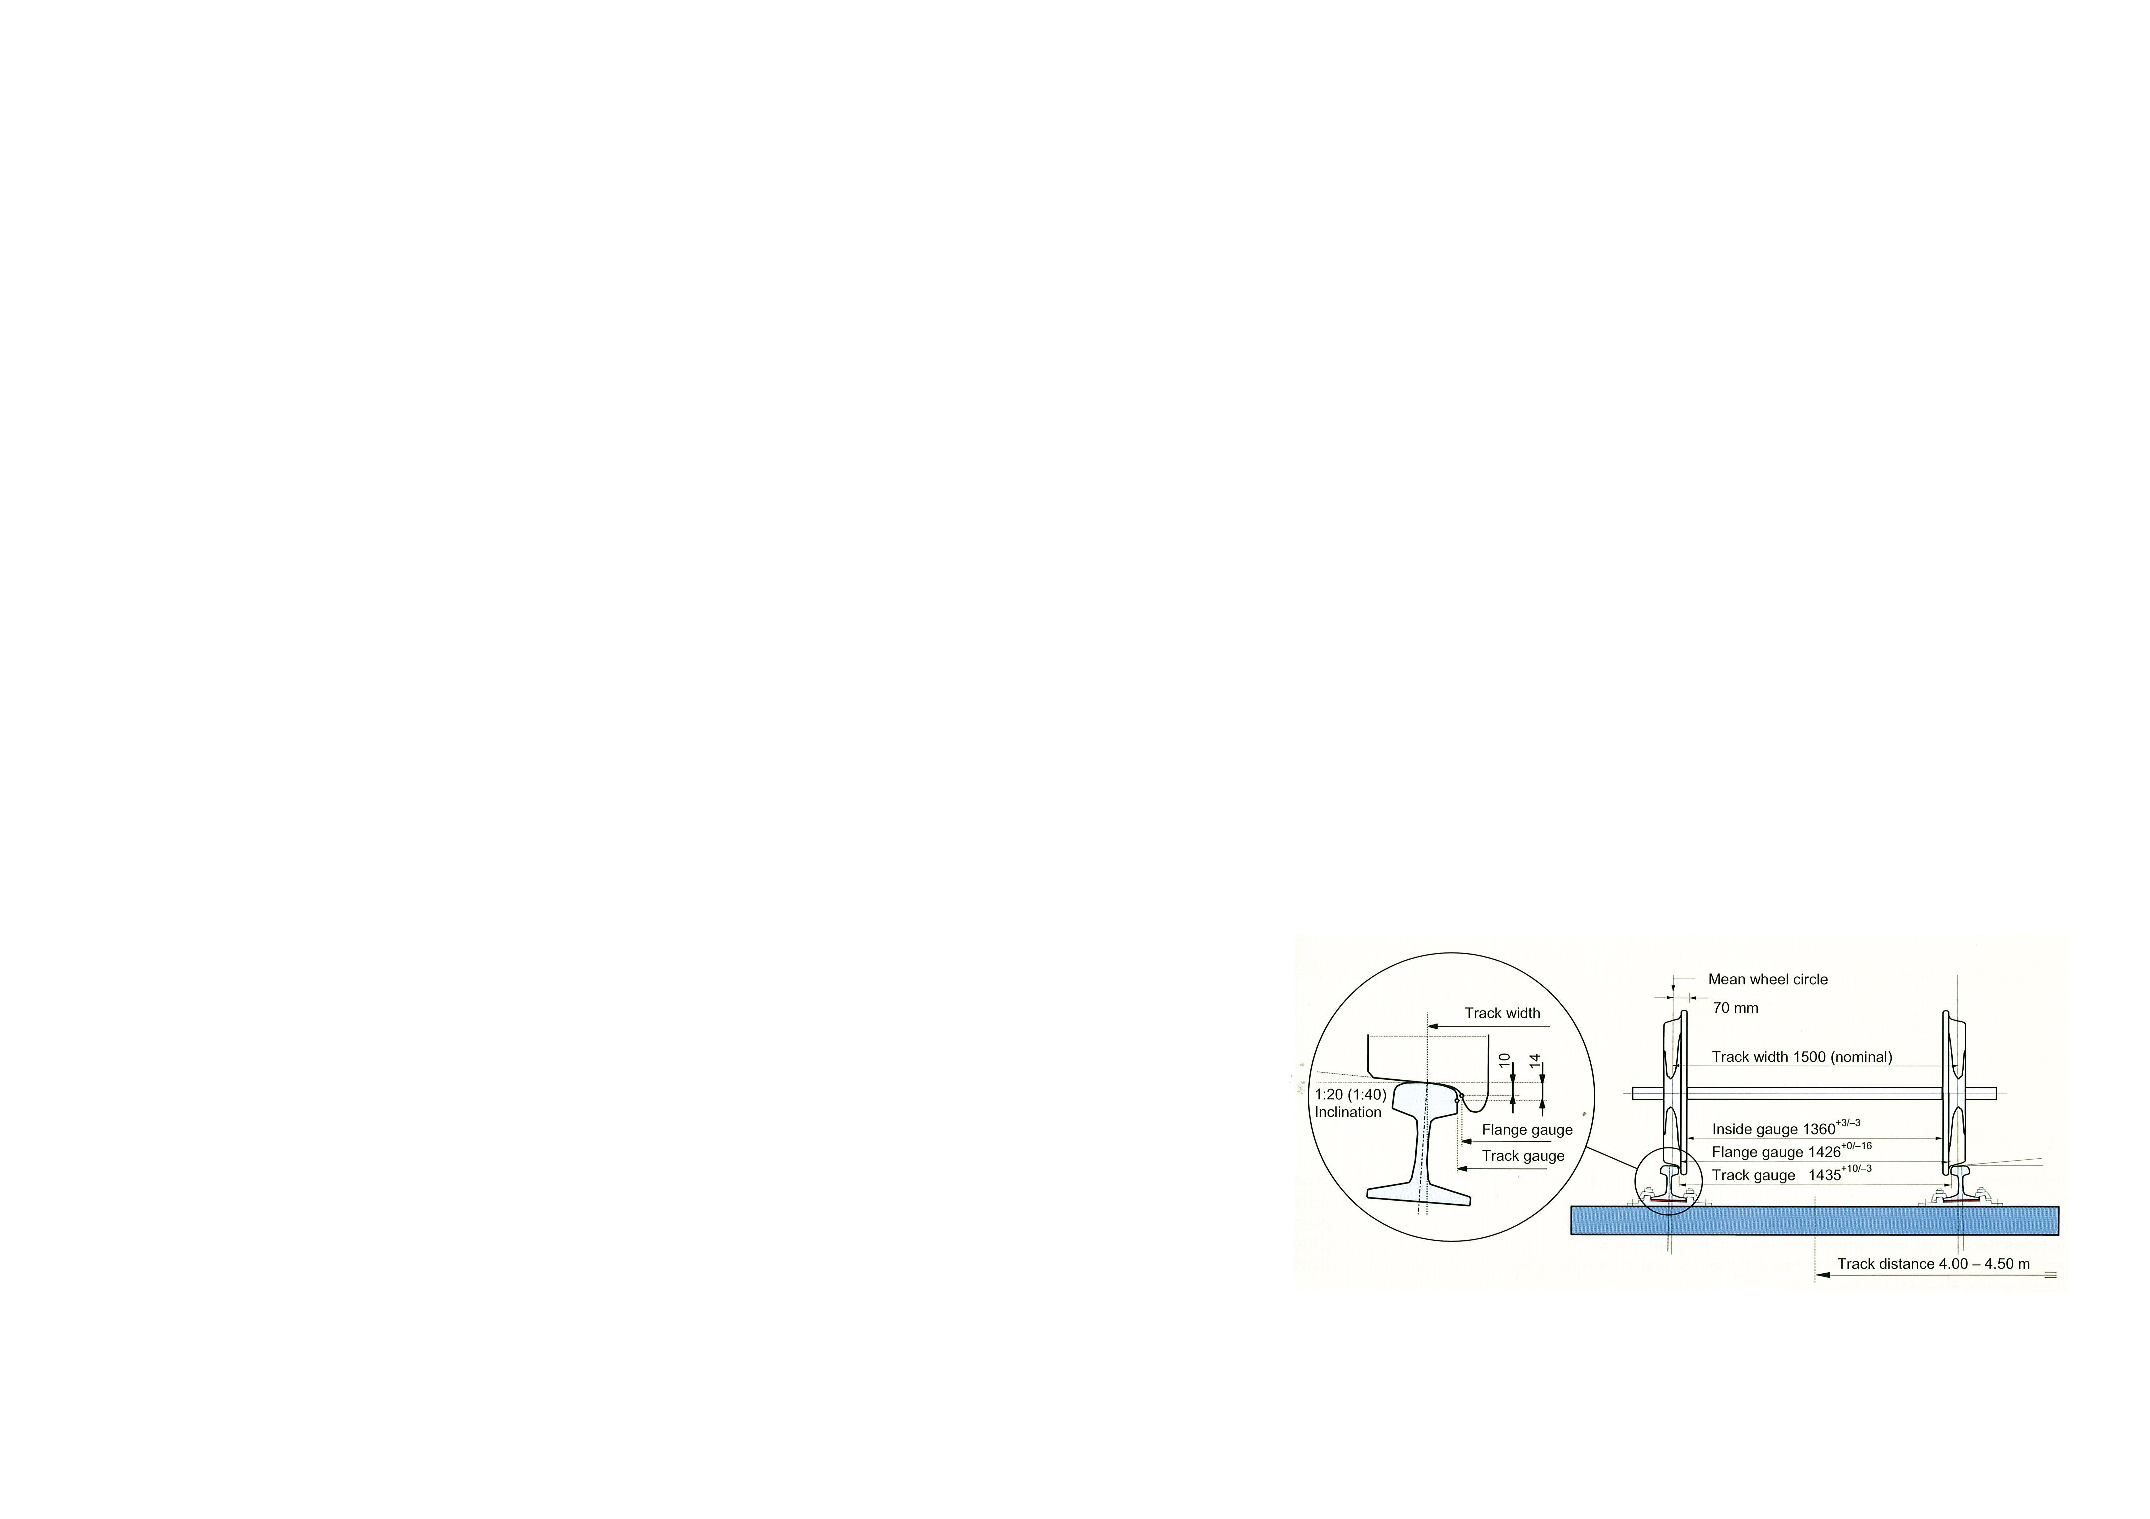
\includegraphics[width=0.5\textwidth]{wheelsettrackdimension.pdf}
\caption{Wheelset and track dimensions. Extracted from \citep[p.17]{esveld2001modern}}
\label{fig:wheelset and track dimensions}
\end{figure}
 
The dimensions of wheelset and track are regulated by International Union of Railways(UIC). Nowadays most of the Dutch rail uses \emph{standard international dimension}. The bridge being designed by Iv-Infra will also apply standard rail dimensions.

The dimension of wheelset and track is explained in Figure.\ref{fig:wheelset and track dimensions}.

Track gauge is defined as a distance between the two rails. On standard track the gauge is $1435^{+10}_{-3}$ mm with with a maximum gradient of $1:3000$. For new track, however, NS apply the following standards\cite{esveld2001modern}:

\begin{enumerate}
\item Mean gauge per 200 m: $1435^{+10}_{-1}$ mm
\item Standard deviation within a 200 m section less than 1 mm
\end{enumerate}

\paragraph{Conicity of wheels and equivalent conicity of wheels}

Conicity of wheels is an important factor influencing the lateral movement of wheelset. Conicity affects the dynamic behavior of wheelsets, therefore affecting the lateral dynamics of the railway vehicles.

The conicity is the inclination of a wheel thread section. Originally conical wheel thread profiles an inclination of 1:20 as shown in Figure.\ref{fig:wheelconicity}. 

\begin{figure}[h!]
	\centering
	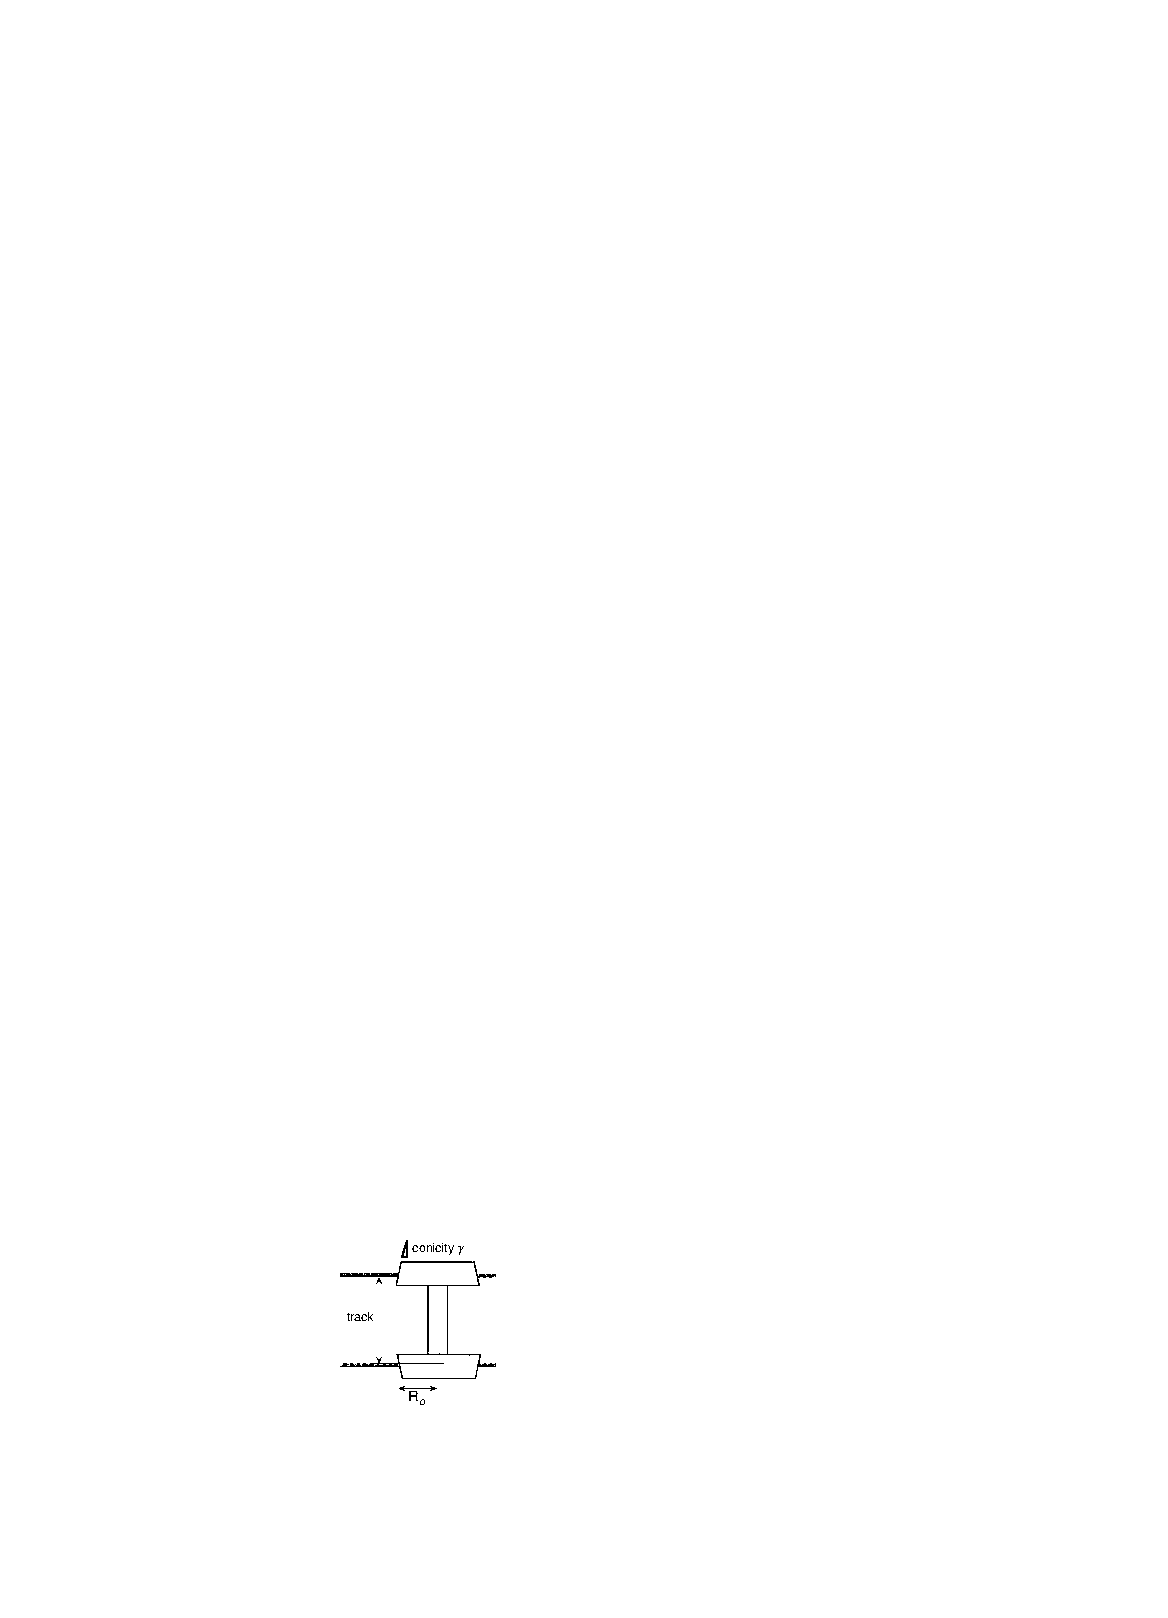
\includegraphics[width=0.3\textwidth]{wheelconicity.pdf}
	\caption{Coning of a wheel thread}
	\label{fig:wheelconicity}
\end{figure}

However, during the manufacturing the tires are given a different shape from a straight conicity. The shape is hollow thus the straight conicity can not effectively describe the geometry of a actual wheel profile. For instance, the S1002 profile defined by UIC is shown in Figure.\ref{fig:s1002}.

\begin{figure}[h!]
	\centering
	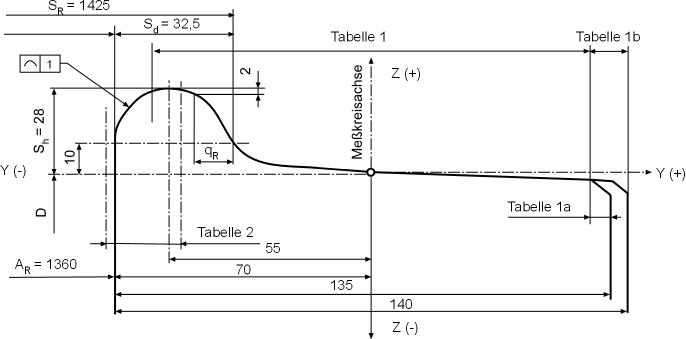
\includegraphics[width=0.5\textwidth]{s1002.jpg}
	\caption{Wheel profile S1002}
	\label{fig:s1002}
\end{figure}

Equivalent conicity is defined to describe the over-all inclination characteristics of a wheel profile. Generally, the equivalent conicity is defined as\cite{esveld2001modern}:

$$ \gamma_e = \frac{\Delta r}{2y} = \frac{r_1 - r_2}{2y}  $$

$r_1 - r_2$ is the instantaneous difference in rolling radius of the wheel treads; generally speaking this is a non-linear function of the lateral displacement y of the wheelset with respect to the central position. 

\paragraph{Worn wheel profiles}

Wheel wears during usage and wheel profiles will change under the effect of wear. Over a period of time wheel profiles stabilize with wear at an equivalent conicity of 0.2 to 0.3\cite{esveld2001modern}. 

\section{Lateral Track Irregularities}
Lateral track irregularities is a source inducing the lateral movement of wheelsets. Track irregularities are minor track deformations that deviate from the original track reference. Well-maintained railway tracks have reduced lateral track irregularities and higher vehicle lateral stability.

The definition is shown in Figure.\ref{fig:lateraldeviationdefine}. See Eurocode\cite{13848} for detailed information about the definition.

\begin{figure}[h]
    \centering
    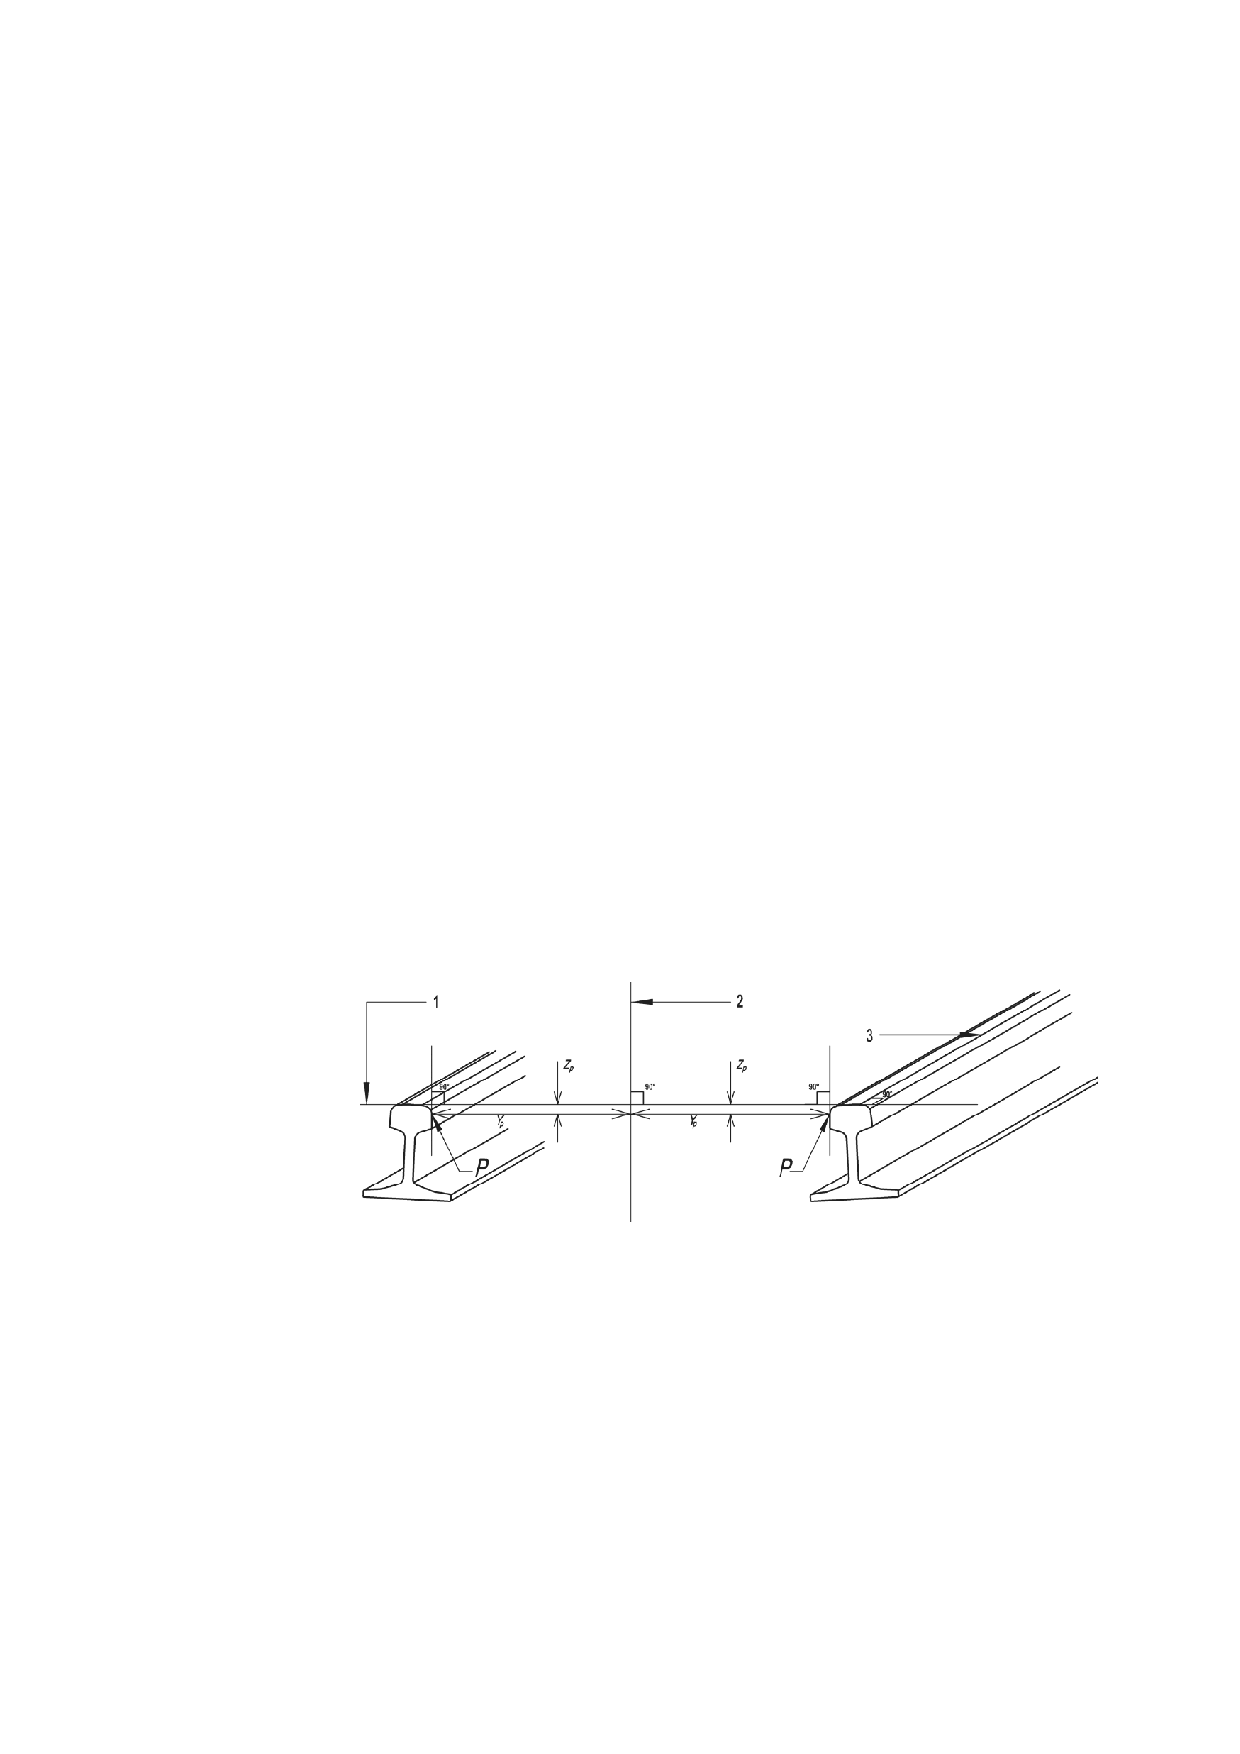
\includegraphics[width=0.8\textwidth]{lateraldeviationdefine}
    \caption{Lateral track irregularity deviation definition\cite{13848}}
    \label{fig:lateraldeviationdefine}
\end{figure}

Table \ref{tab:lateraldeviation}\cite{13848} defines the allowable standard deviation for lateral track irregularities. 

\begin{table}[h]
    \centering
    \caption{Lateral standard deviation\citep[Extracted from][Table B.6]{13848}}
    \begin{tabular}{cc}
        \hline
        Speed(km/h) & Standard deviation(mm) \\
        \hline
        $V\leq 90$ & 1.5 to 1.8 \\
        $80 < V \leq 120$ & 1.2 to 1.5 \\
        $120 < V \leq 160$ & 1.0 to 1.3 \\
        $160 <V \leq 230$ & 0.8 to 1.1 \\
        $230 <V \leq 300$ & 0.7 to 1.0 \\
        \hline
    \end{tabular}
    \label{tab:lateraldeviation}
\end{table}

\section{Lateral movement of wheelsets}
Lateral movement of wheelsets is an essential topic to lateral dynamics of railway bridge because lateral loads on bridge are in direct consequence of lateral movement of wheelsets. 

\paragraph{Contact between wheel and rail}

The movement characteristics of wheels depends on the contact type. There are two types of wheel-rail contact: single-point contact and two-point contact.

In the case of single-point contact, according to Figure.\ref{fig:singlecontact}, wheel load and lateral force act on the same point. This situation occurs when using worn wheel profiles. In the case of two-point contact, shown in Figure.\ref{fig:doublecontract}, the application points do not coincide.

Flanging occurs in the situation of two-point contact. 

\begin{figure}[h!]
\centering
    \begin{subfigure}[b]{0.2\textwidth}
        \centering
        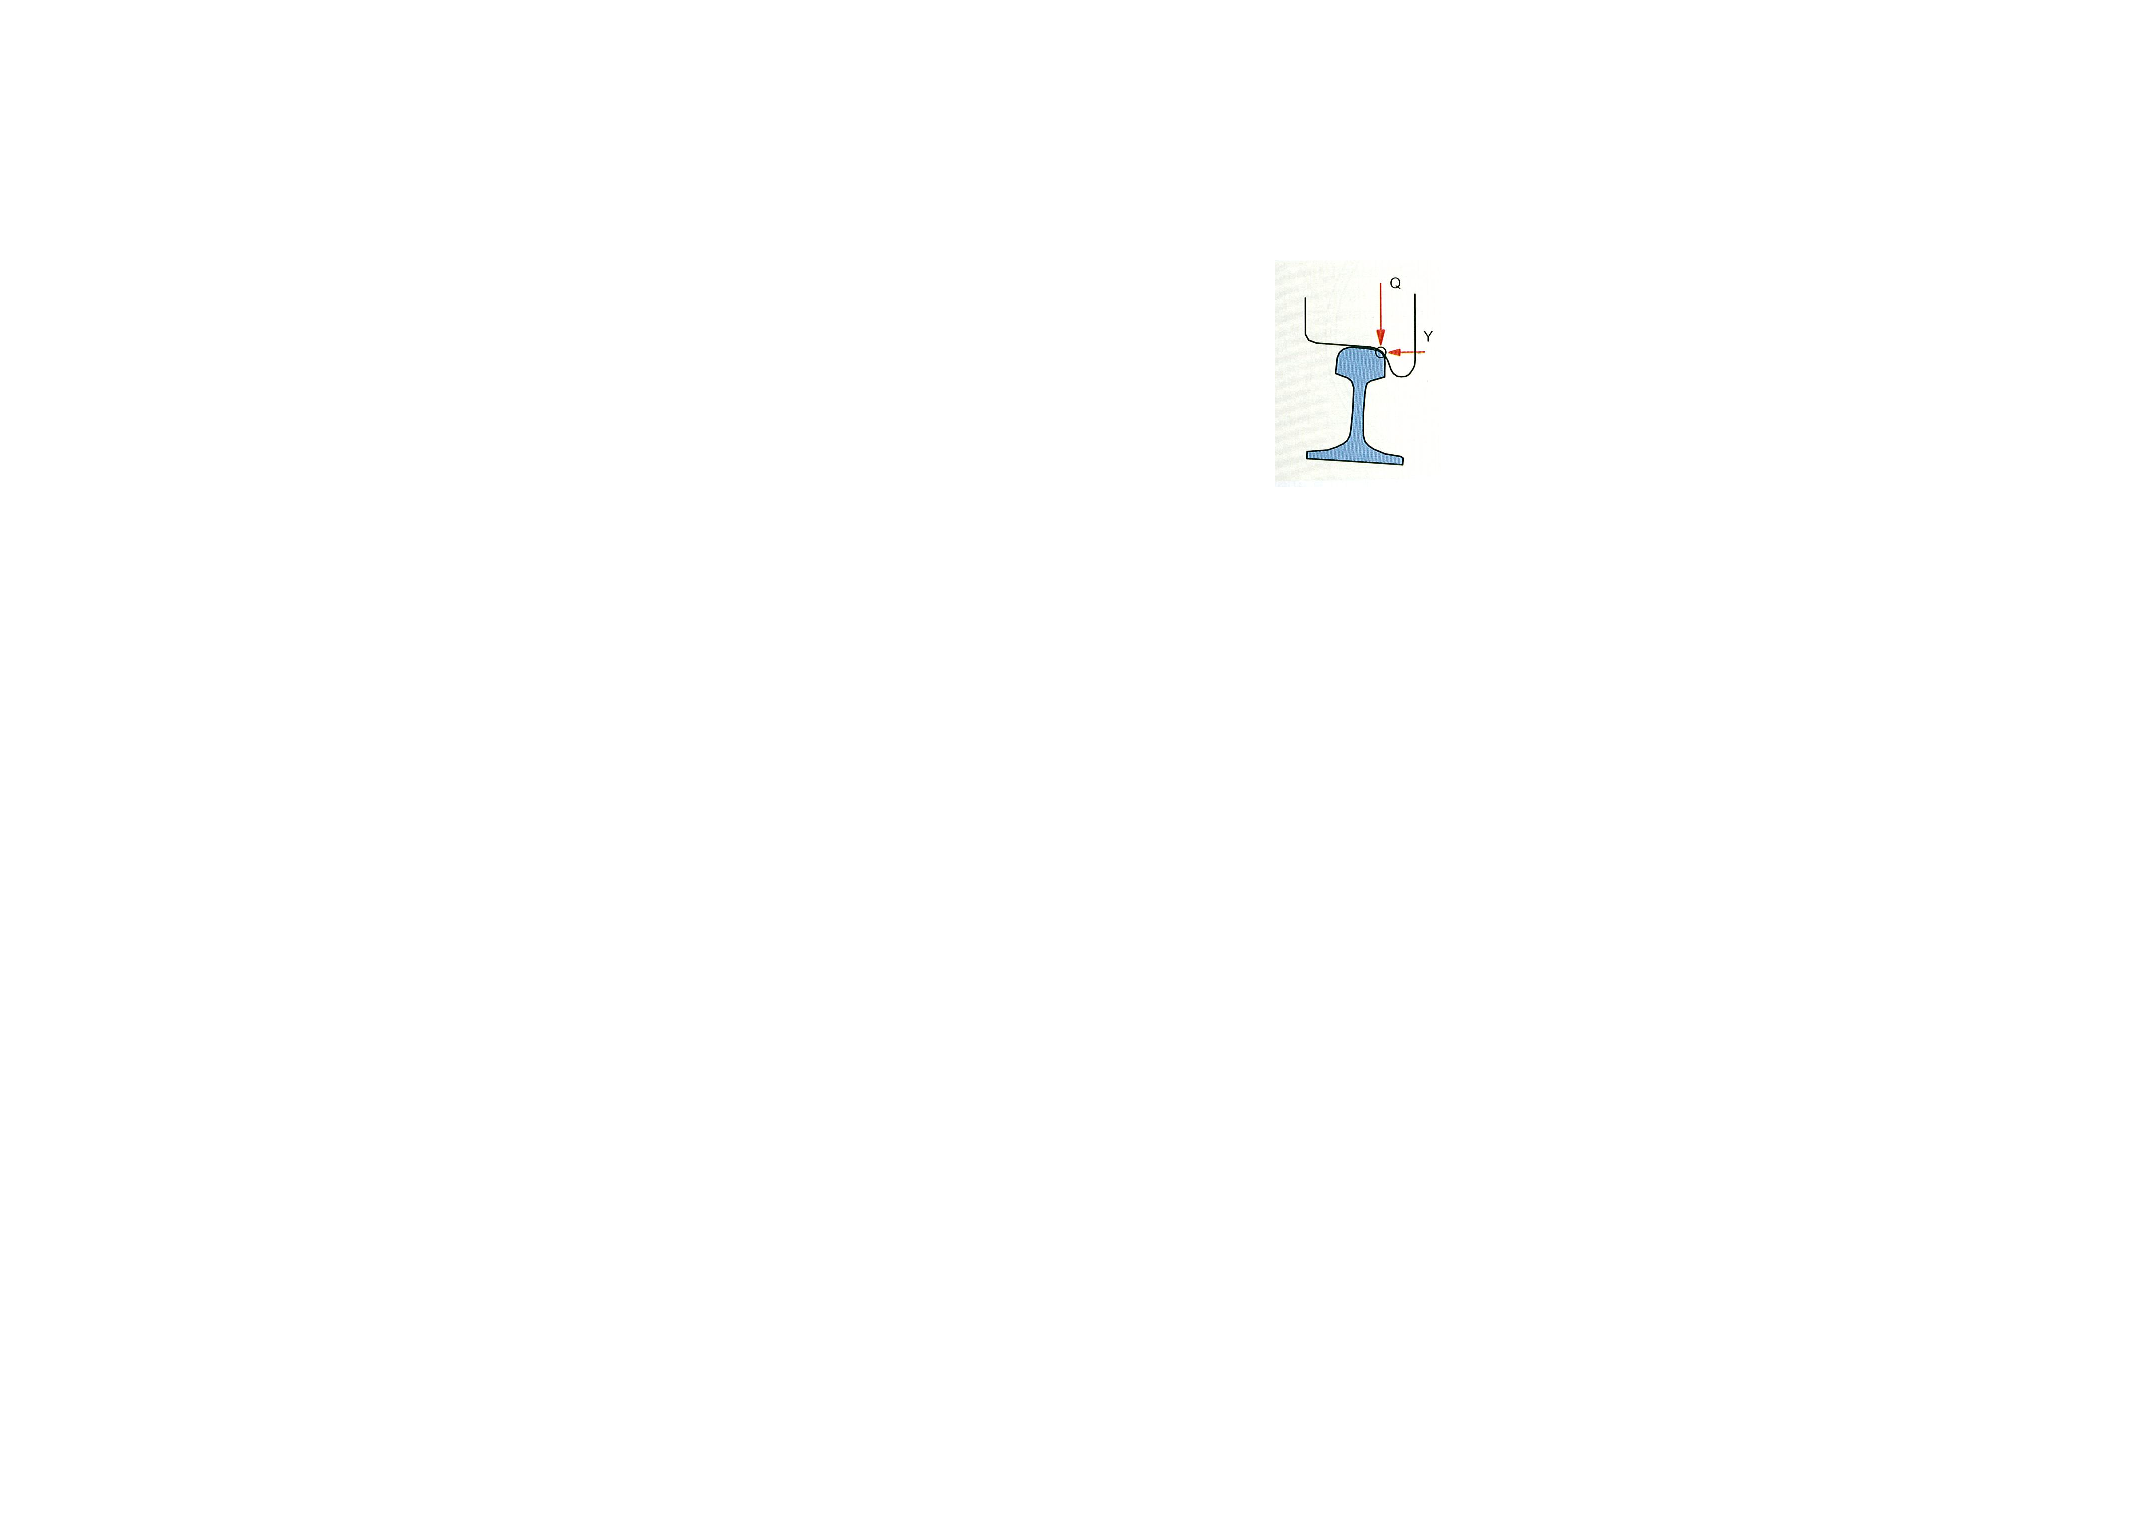
\includegraphics[width=\textwidth]{singlecontact}
        \caption{Single contact point.  Extracted from \citep[Figure 2.13]{esveld2001modern}}
        \label{fig:singlecontact}
    \end{subfigure}
    \begin{subfigure}[b]{0.5\textwidth}
        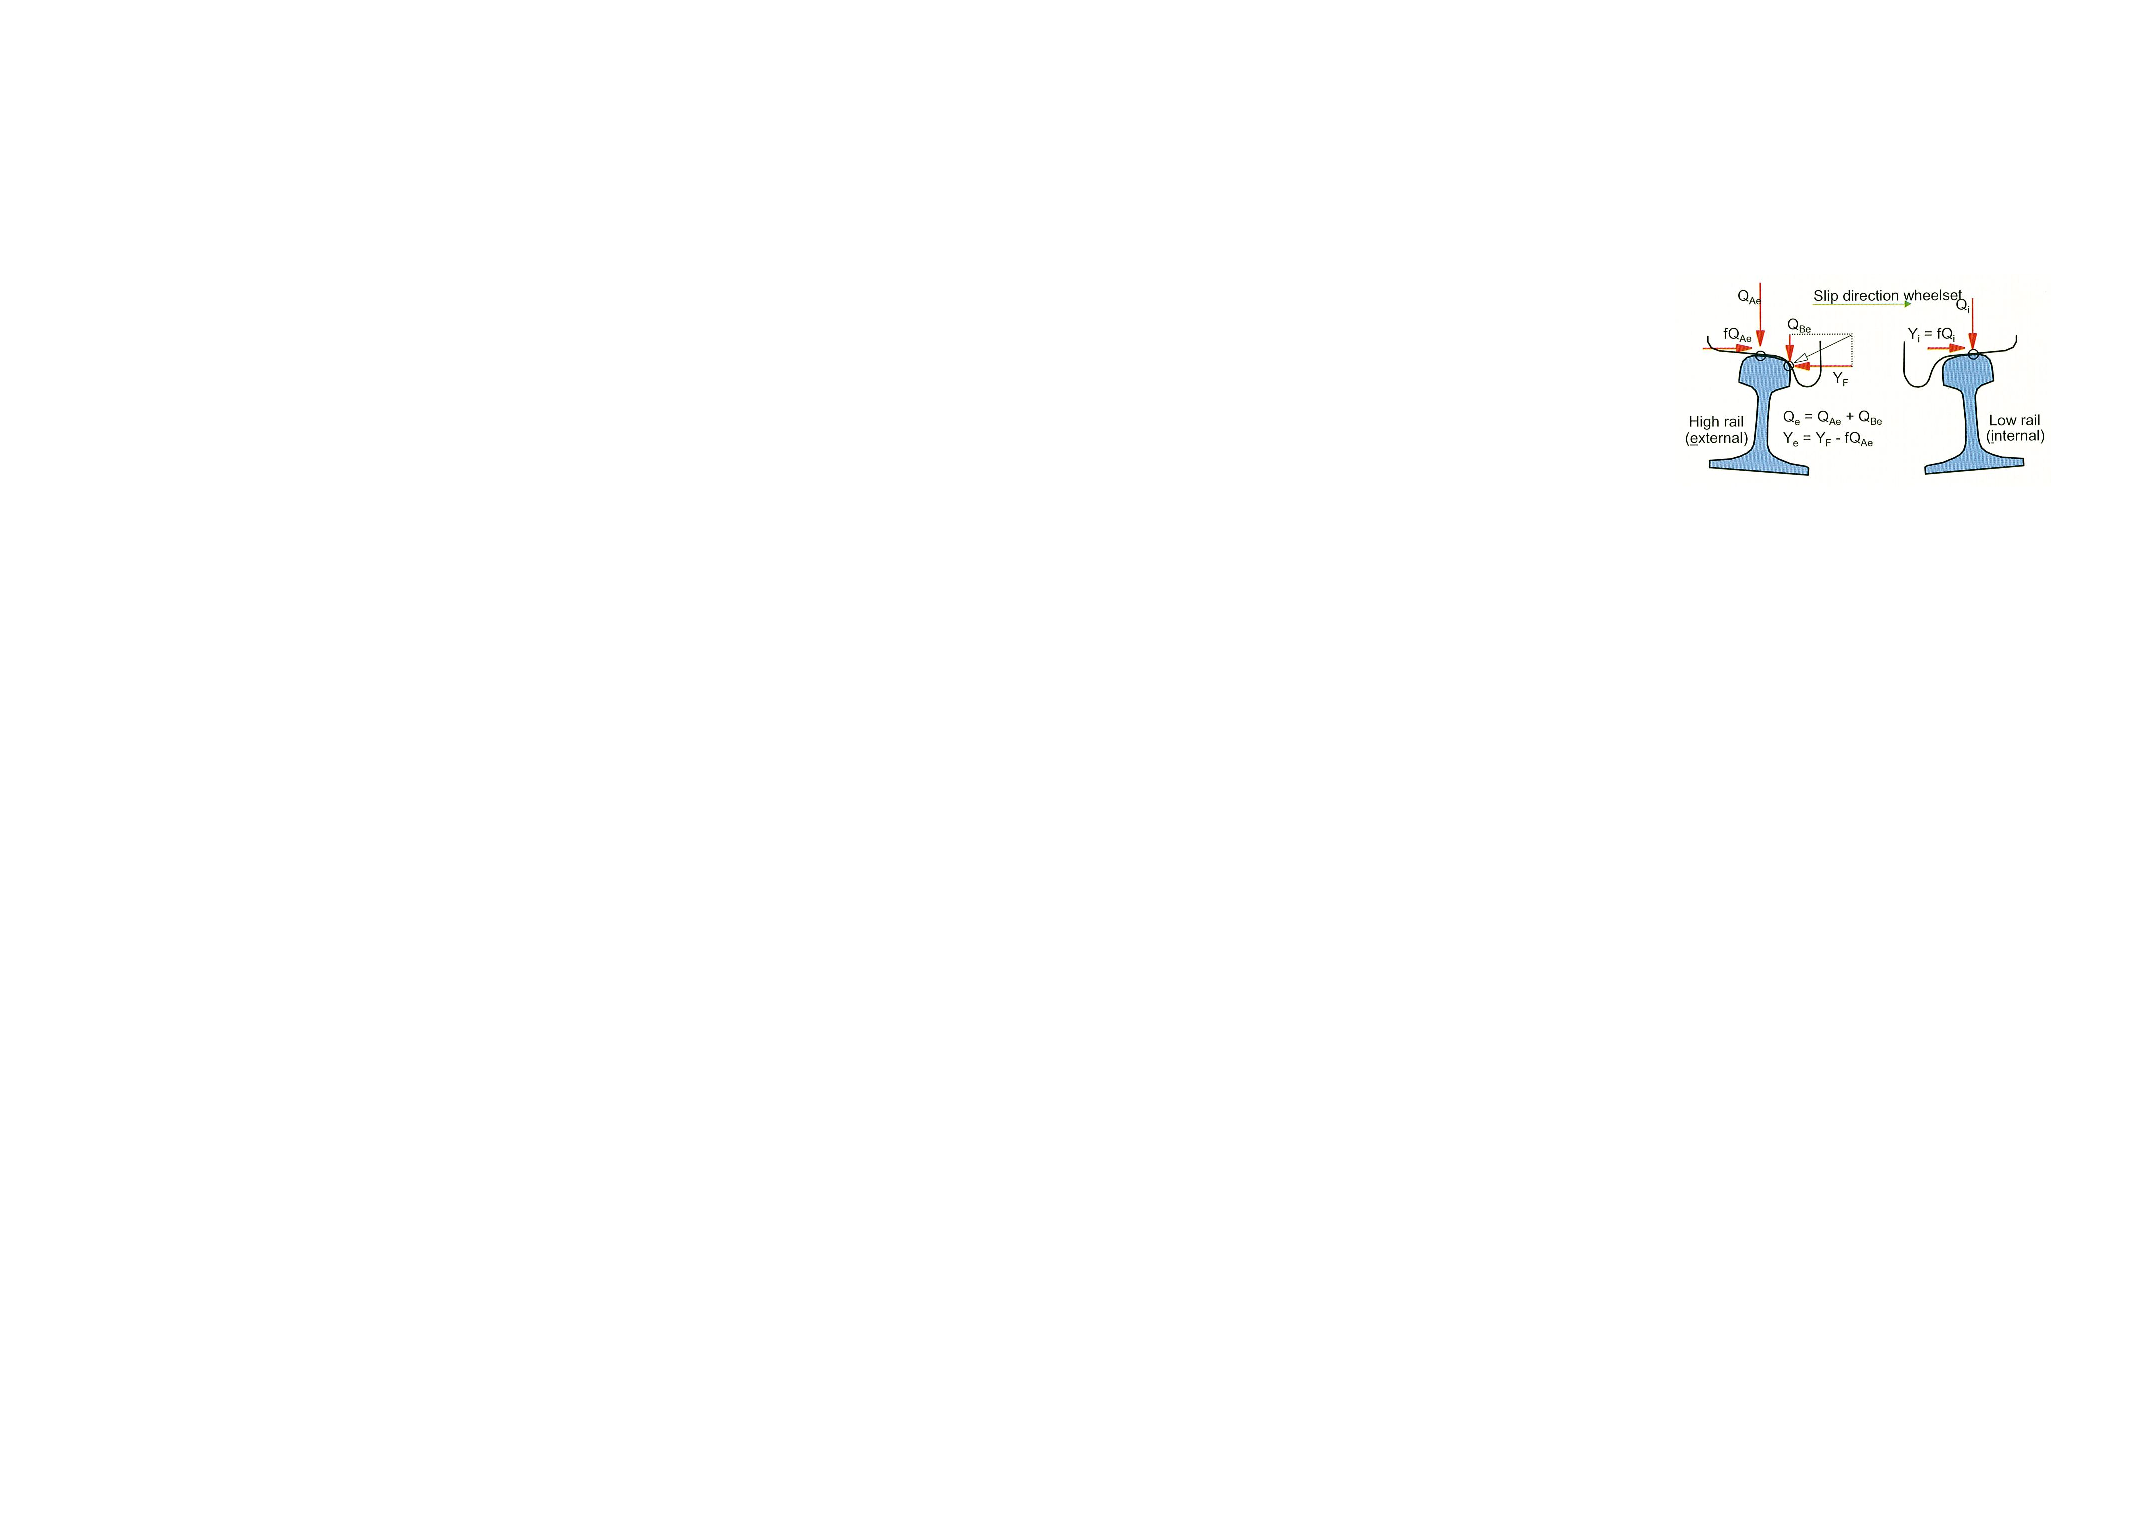
\includegraphics[width=\textwidth]{doublecontact}
        \caption{Double contact points. Forces on rails in case of lateral slip in curves. Extracted from \citep[Figure 2.14]{esveld2001modern}}
        \label{fig:doublecontract}
    \end{subfigure}
    \caption{Single and double contact of wheel-rail interface}
\end{figure}

\paragraph{Klingel movement}

The Klingel movement happens under single-point contact.

Klingel described a periodical movement of the wheelset with conical tire profiles, which is also know as Klingel movement. It was assumed that the wheelset is laterally displaced from central position and the track is ideally straight. This displacement is expected to be counteracted due to different rolling radii of wheels. 

Analysis visualizes the Klingel movement, shown in Figure.\ref{fig:klingelmovement}. The lateral displacement $y$ is a harmonic, undamped function of the distance co-ordinate $x$ as long as the amplitude moves within the wheel flangeway clearance. However, it should be noted that forces play no part in the derivation. Thus Klingel movement is purely a kinematic movement.

\begin{figure}[h]
    \centering
    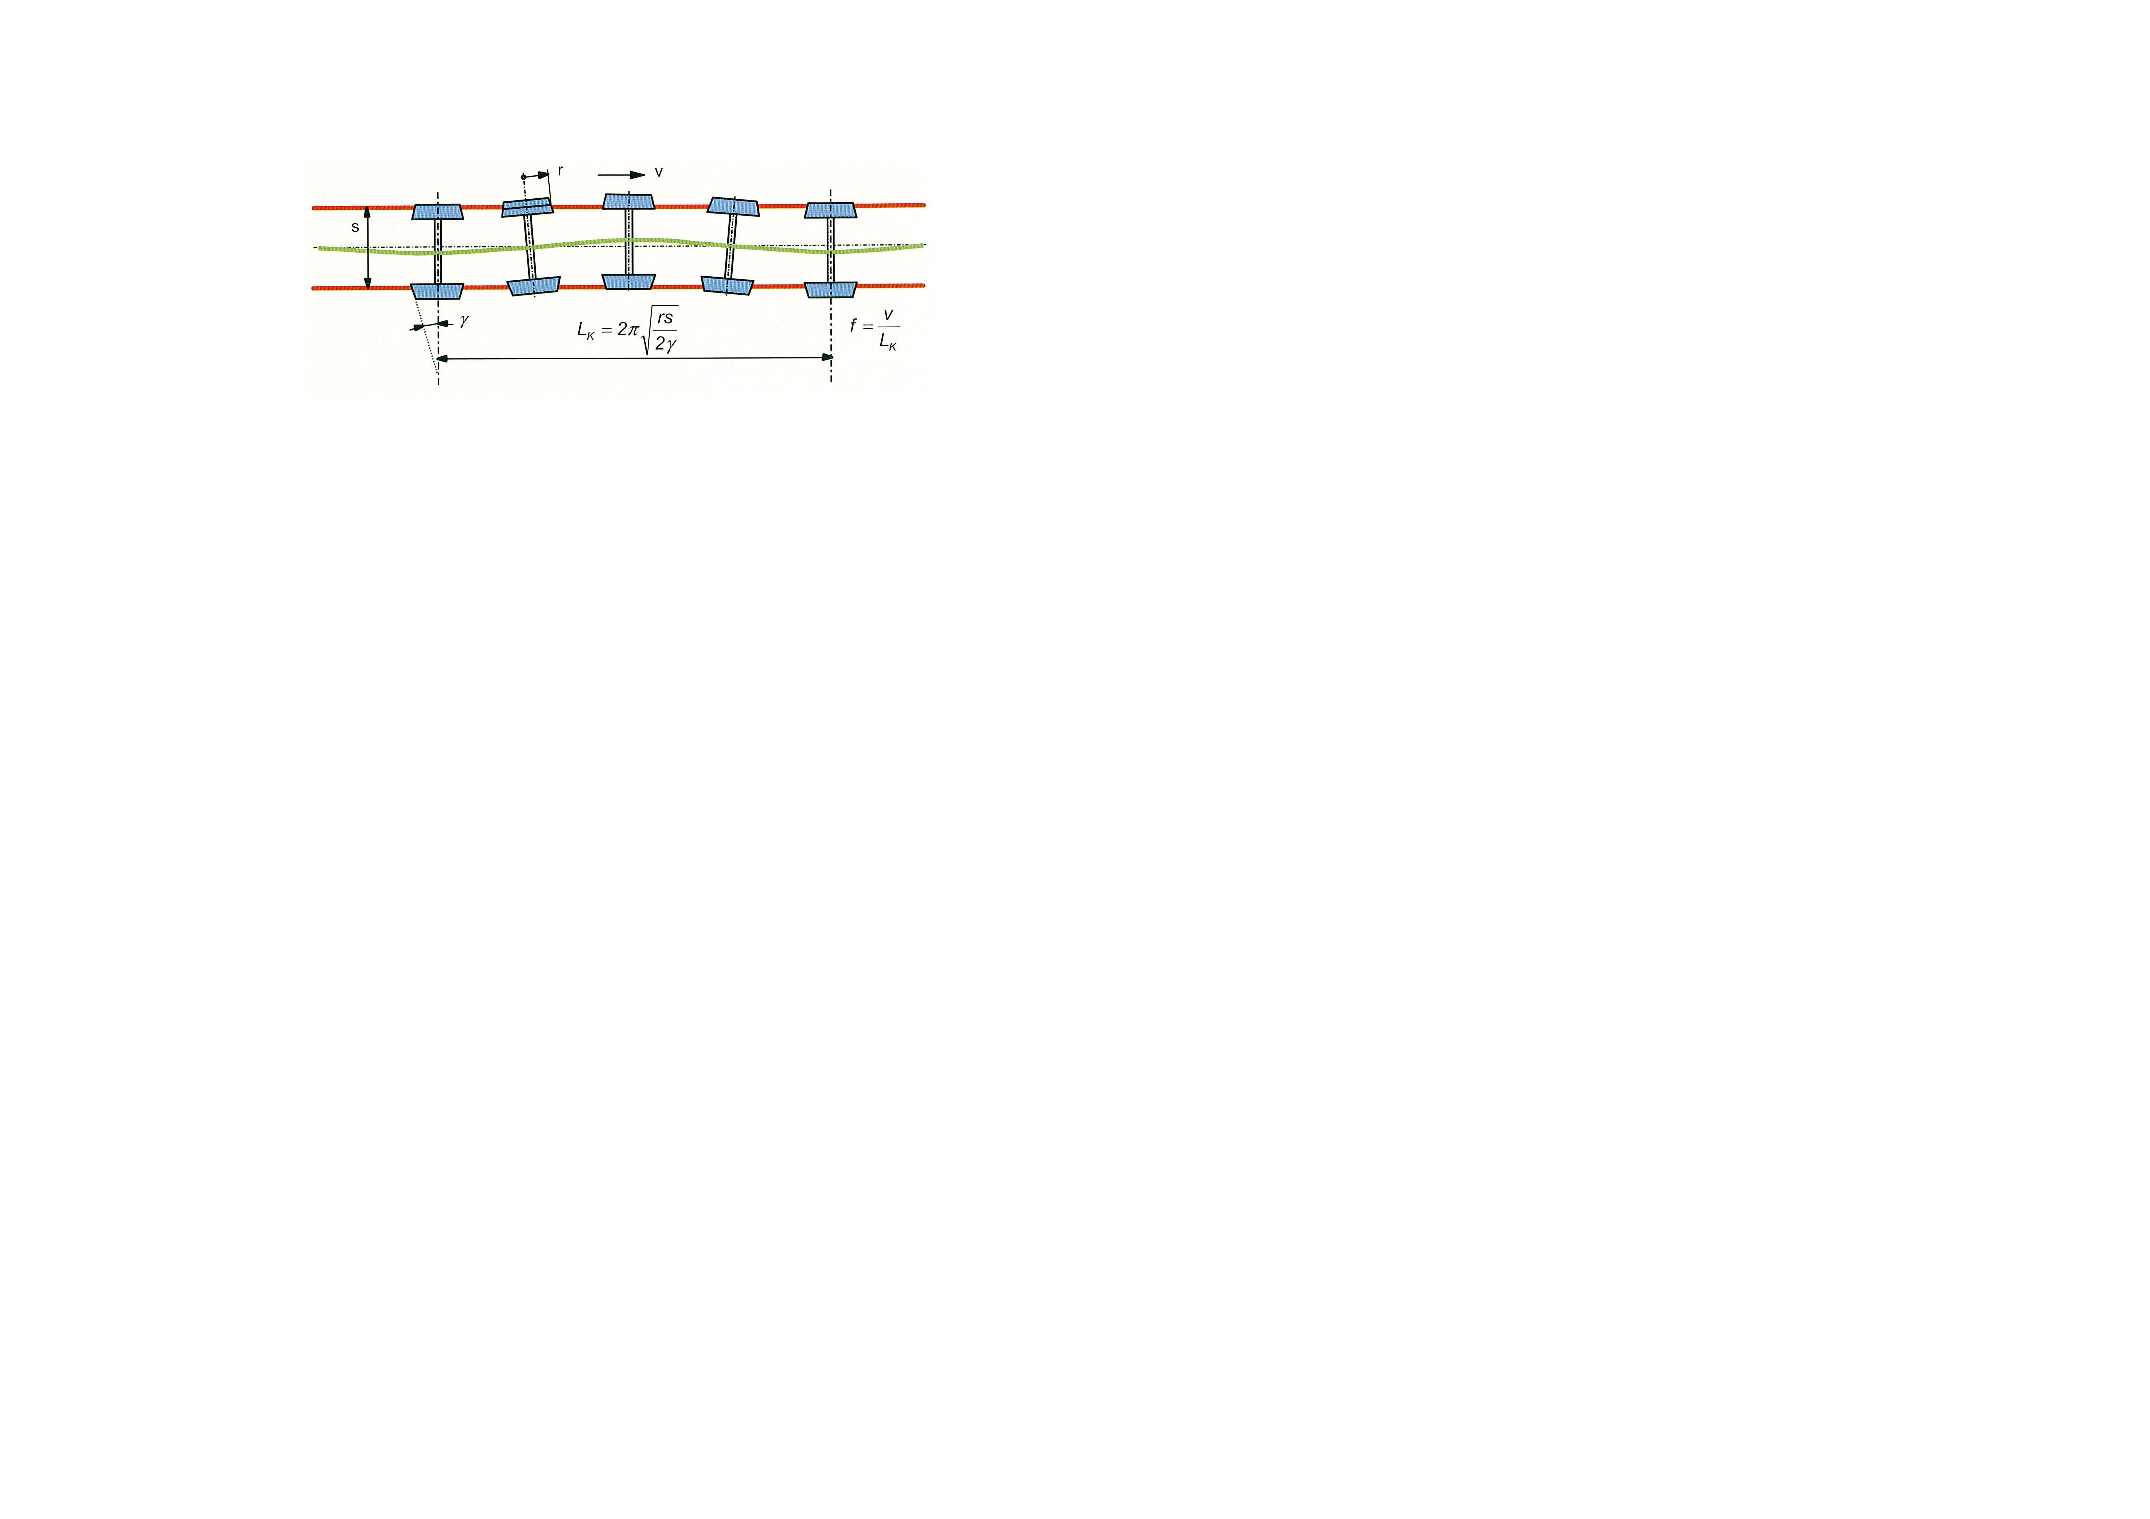
\includegraphics[height = 3cm]{klingelmovement}
    \caption{Klingel movement. Extracted from \citep[Figure 2.3]{esveld2001modern}}
    \label{fig:klingelmovement}
\end{figure}

The expression for wavelength of Klingel movement is shown in Eq.\ref{eq:klingelwavelength}.

\begin{figure}[h]
	\centering
	\begin{equation}
		\label{eq:klingelwavelength}
		L_k = 2\pi\sqrt{\frac{rs}{2\gamma}}
	\end{equation}
	\begin{tabular}{@{}>{$}l<{$}l@{}}
		where: & \\
		L_k & Wavelength of Klingel movement \\
		r & Radius of wheels \\
		s & Gauge distance \\
		\gamma & Conicity of wheels \\
	\end{tabular}
\end{figure}

Introducing the speed, the frequency of Klingel movement is Eq.\ref{eq:klingelfrequency}.

\begin{equation}\label{eq:klingelfrequency}
	f = \frac{V}{L_k} 
\end{equation}

\paragraph{Hunting movement}
The hunting movement happens under two-point contact. Flanging happens in hunting movement.

It should be noted that the Klingel theory is simple and instructive but does not include the effect of coupled axes, mass forces, and adhesion forces. In reality, the amplitude $y_0$ of the Klingel movement is dependent on alignment, dynamic vehicle behavior, and the speed of the rolling stock. 

Generally speaking, $y_0$ due to slip will increase with speed until it is equal to half the flangeway clearance. Flanging then occurs as a result of which the axle will rebound. 

This means that the lateral movement takes on a completely different behavior which is known as hunting. As shown in the drawing in Figure\ref{fig:flangingwheelset} the movement changes from a harmonic to a zig-zag shape. The wavelength becomes shorter and the frequency increases quickly as hunting effect builds up.

\begin{figure}[h]
    \centering
    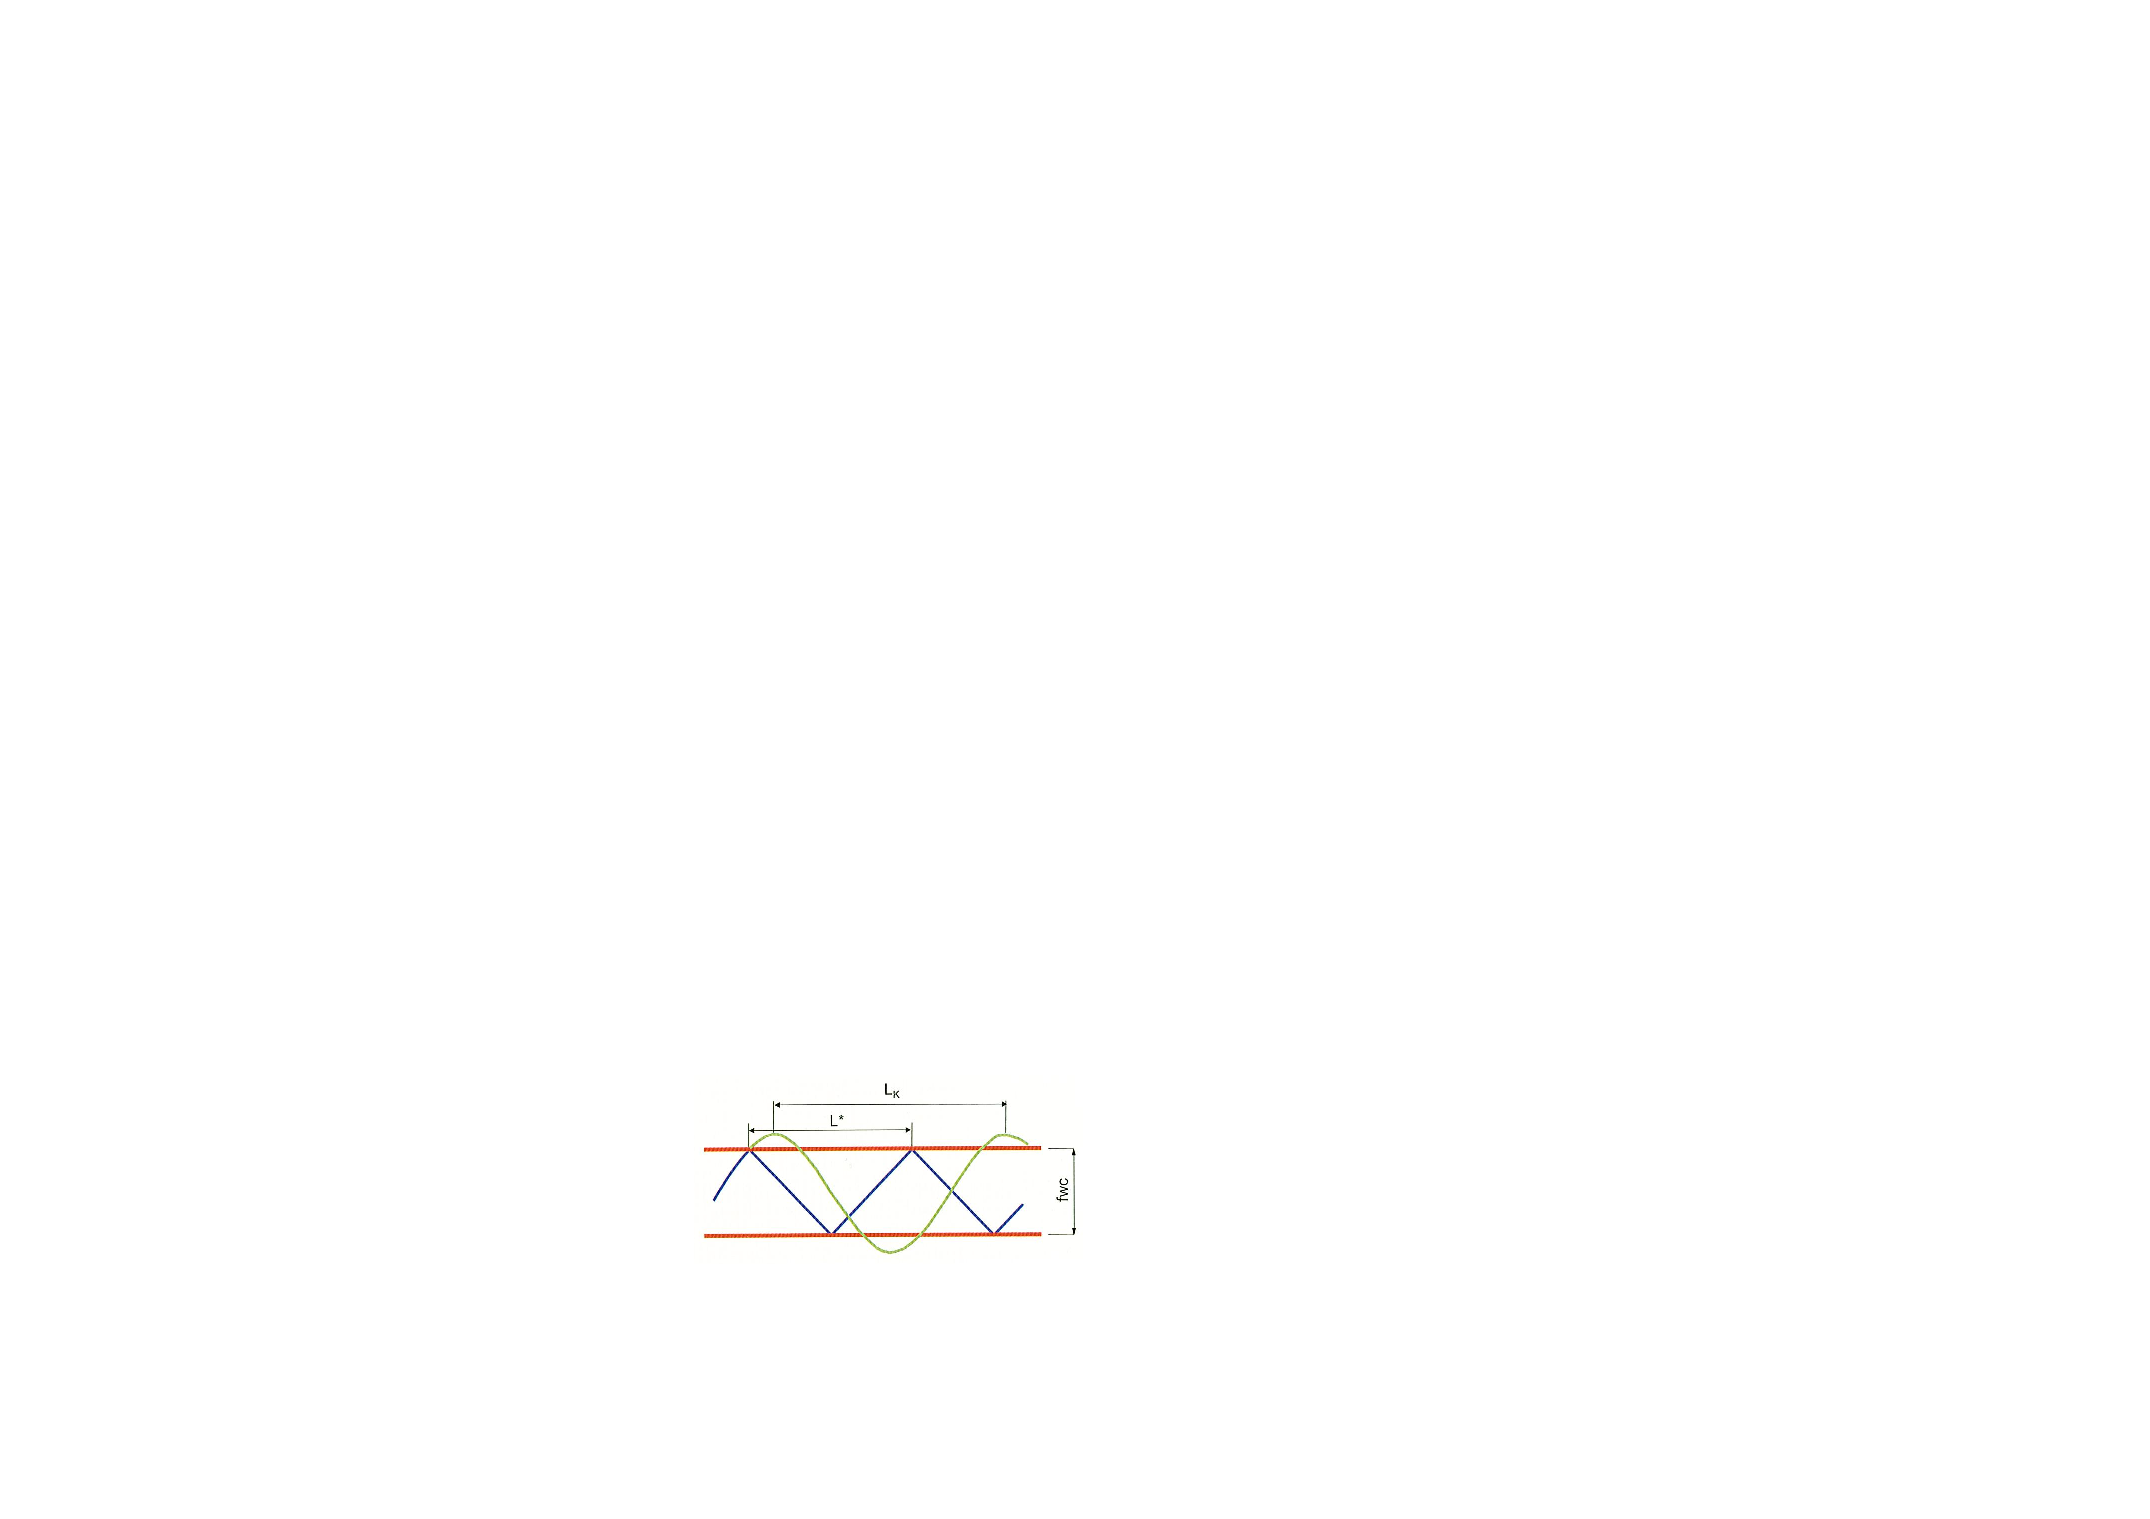
\includegraphics[width=0.5\textwidth]{flangingwheelset}
    \caption{Influence of flanging on lateral wheelset movement. Extracted from \citep[Figure 2.5]{esveld2001modern}}
    \label{fig:flangingwheelset}
\end{figure}

\section{Bridge natural frequency}
The natural frequency of a bridge is an important characteristics of its structural dynamics. 

Research\citep{reberpresentation} shows simplified method can be used to predict the natural frequencies of a bridge. The bridge is modeled as a uniform, simply supported beam. It is validated that the natural frequency of the beam approximately equals to the natural frequency of the bridge.

The beam is simply supported at both ends, and the stiffness of the beam is specified as a deflection at the mid span per unit span length arising from a static point load of 100kN at mid span on the bridge. The length of the beam equals to the span of the bridge. The total mass of the bridge is uniformly distributed over the beam.

The derived natural frequencies of the bridge is shown in Eq.\ref{eq:beamnaturalfrequency}. 

\begin{figure}[h]
	\centering
	\begin{equation}
		\label{eq:beamnaturalfrequency}
		f_r = \frac{r^2 \pi}{2L^2}\sqrt{\frac{EI}{m}}
	\end{equation}
	\begin{tabular}{@{}>{$}l<{$}l@{}}
		where: & \\
		r & Natural mode:1,2,3... \\
		L & Span of the bridge \\
		EI & Equivalent stiffness of the bridge\\
		m & Mass per unit length of the bridge \\
	\end{tabular}
\end{figure}

\section{Lateral vehicle-bridge resonance}
The resonance mechanism between railway vehicle and bridge is a complicated topic. Two types of vehicle-bridge resonance have been validated to be possible by UIC\citep{d181dt329}. They are:

\begin{enumerate}
    \item Resonance caused by axle repeat pattern
    \item Resonance caused by kinematic movement
\end{enumerate}

\paragraph{Resonance caused by axle repeat pattern}
Axle repeat pattern is the periodic pattern of train axles passing on a fixed location. The axle repeat pattern introduces forces to rail track on both vertical and lateral direction. 

The wavelength of the axle repeat pattern is only dependent on the layout of the train. Although the distance between any two axles can form a wavelength, due to the regular arrangement coaches/wagons, there are only a few dominant wavelength. 

Since frequency is speed divided by wavelength, the frequency of the axle repeat patterns vary with train speed. A table of axle repeat pattern lengths, and typical frequencies arising from train speed are given in Figure.\ref{tab:329axlerepeat}

Research\citep[3.4.3]{d181dt329} shows that by running train at different speeds, resonance is possible between train and bridge if the axle passing frequency coincides with the first lateral bridge mode. The resonance effect is more pronounced compared to kinematic movement resonance\citep[Chapter 5, Research Phase II]{d181dt329}.

\paragraph{Resonance caused by kinematic movement}
The lateral kinematic movement of railway vehicles is also wavelength phenomenon. However, the wavelength of lateral kinematic movement is much more complicated than axle repeat pattern. Many factors affect the wavelength of vehicle lateral kinematic movement. These factors include track irregularities, wheel profile, rail profile and other factors that may influence the lateral movement of wheelsets.

The lateral kinematic wavelength of railway vehicles are hard to predict. Research\citep{d181dt329} obtains the lateral kinematic wavelength of the vehicle by numerical modeling a running railway vehicle. 

The frequency of kinematic movement resonance is speed divided by wavelength. By coinciding the lateral kinematic frequency of the vehicle and bridge first lateral natural frequency, the resonance caused by kinematic movement was successfully validated\citep{d181dt329}.

 